% Drawing 144/03-3 -- folder 144, batch 03, archive page 52 (PDF page 53).
% Transcription: Un morceau de carte trivalente (traits gras) et, en traits fins au crayon, sa subdivision barycentrique. Au sommet $s$ de la carte, le long de l'arête $a$ (flèche $\to a$) et dans la face $f$, le triangle hachuré de sommets $s$, $\tilde a$ (centre de $a$) et $\tilde f$ (centre de $f$) est le repère $r$ ; une flèche courbe indique le sens de rotation du repère, une flèche verticale l'orientation normale.
% Kind: trivalent map with barycentric subdivision and a hatched frame. Method 2 (schematic redraw from the facsimile). Status: ok.
% Notes: Bold: edges of the trivalent map; pencil: two strokes of the barycentric subdivision. The hatched triangle s, a~, f~ is the frame r, with a curved rotation arrow and the vertical arrow of the normal orientation; the thin arrow from s along the edge is "-> a". Several pencil strokes of the subdivision are too faint to place and are not drawn.
% Coordinates: 1 unit = 1 mm = 1/100 of the crop width (bbox in page fractions: [0.24, 0.24, 0.5, 0.43]).
% Redrawn by Claude (claude-opus-5-5), issue #73, 2026-11-07; not checked by a human; not compiled (no TeX in the session).
% Rights: reproduces part of the work -- behind RENDER_TRANSCRIPTS, never published by itself.
\documentclass[tikz,border=3pt]{standalone}
\usepackage{amsmath,amssymb}
\usetikzlibrary{patterns,arrows.meta}
\tikzset{pencil/.style={black!45}, struck/.style={black!35}, mark/.style={circle,draw,inner sep=1.3pt}, pt/.style={circle,fill,inner sep=0.9pt}, opt/.style={circle,draw,fill=white,inner sep=1.1pt}}
\begin{document}
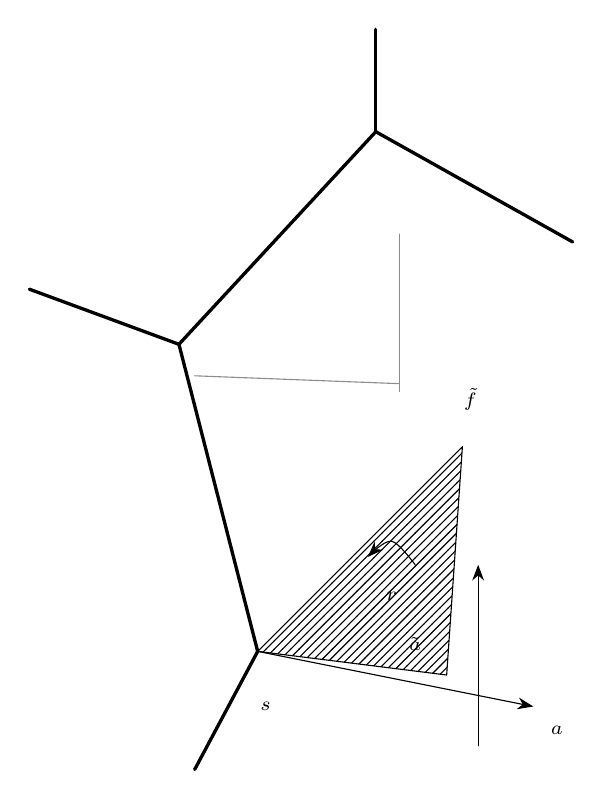
\begin{tikzpicture}[x=1mm,y=1mm,line cap=round,line join=round,font=\scriptsize]
\draw[very thick] (75,-4) -- (75,-17);
\draw[very thick] (75,-17) -- (100,-31);
\draw[very thick] (75,-17) -- (50,-44);
\draw[very thick] (50,-44) -- (31,-37);
\draw[very thick] (50,-44) -- (60,-83);
\draw[very thick] (60,-83) -- (52,-98);
\draw[pencil] (78,-30) -- (78,-50);
\draw[pencil] (52,-48) -- (78,-49);
\draw (60,-83) -- (86,-57) -- (84,-86) -- cycle;
\fill[pattern=north east lines] (60,-83) -- (86,-57) -- (84,-86) -- cycle;
\draw[-{Stealth[length=2mm]}] (60,-83) -- (95,-90);
\draw[-{Stealth[length=2mm]}] (88,-95) -- (88,-72);
\draw[-{Stealth[length=2mm]}] plot[smooth, tension=0.55] coordinates {(80,-72) (77,-69) (74,-71)};
\node[inner sep=1pt] at (61,-90) {\scriptsize $s$};
\node[inner sep=1pt] at (77,-76) {\scriptsize $r$};
\node[inner sep=1pt] at (80,-82) {\scriptsize $\tilde a$};
\node[inner sep=1pt] at (87,-51) {\scriptsize $\tilde f$};
\node[inner sep=1pt] at (98,-93) {\scriptsize $a$};
\end{tikzpicture}
\end{document}
